\documentclass[11pt,twocolumn,a4paper]{article}

\usepackage[utf8]{inputenc}
\usepackage[T1]{fontenc}
\usepackage{amsmath,amssymb,amsthm,amsfonts}
\usepackage{mathtools}
\usepackage{geometry}
\usepackage{graphicx}
\usepackage{booktabs}
\usepackage{hyperref}
\usepackage{algorithm}
\usepackage{algpseudocode}
\usepackage{natbib}
\usepackage{cleveref}
\usepackage{tikz}
\usetikzlibrary{positioning,arrows.meta,shapes.geometric,fit,backgrounds}
\usepackage{xcolor}
\usepackage{bbm}

\geometry{margin=1in}

\newtheorem{theorem}{Theorem}[section]
\newtheorem{proposition}[theorem]{Proposition}
\newtheorem{lemma}[theorem]{Lemma}
\newtheorem{corollary}[theorem]{Corollary}
\theoremstyle{definition}
\newtheorem{definition}[theorem]{Definition}
\newtheorem{assumption}[theorem]{Assumption}
\theoremstyle{remark}
\newtheorem{remark}[theorem]{Remark}
\newtheorem{example}[theorem]{Example}

\DeclareMathOperator*{\argmin}{arg\,min}
\DeclareMathOperator*{\argmax}{arg\,max}
\newcommand{\R}{\mathbb{R}}
\newcommand{\N}{\mathbb{N}}
\newcommand{\Z}{\mathbb{Z}}
\newcommand{\E}{\mathbb{E}}
\renewcommand{\Pr}{\mathbb{P}}
\newcommand{\MSI}{\mathsf{MSI}}
\newcommand{\Lc}{\mathcal{L}}
\newcommand{\Cc}{\mathcal{C}}
\newcommand{\Sc}{\mathcal{S}}
\newcommand{\Uc}{\mathcal{U}}
\newcommand{\Mc}{\mathcal{M}}
\newcommand{\Xc}{\mathcal{X}}
\newcommand{\Fc}{\mathcal{F}}

\title{The Minimum Sufficient Interceptor:\\
Natural-Language-to-Coordinate Mediation\\
at the Operating System Boundary}

\author{
Kundai Farai Sachikonye\\
AIMe Registry for Artificial Intelligence\\
\texttt{kundai.sachikonye@wzw.tum.de}
}

\date{\today}

\begin{document}
\maketitle

\begin{abstract}
Contemporary systems increasingly position a general-purpose large language model (LLM) at the boundary between human natural-language input and a structured computational substrate. Such a model typically performs three distinct functions simultaneously: it parses user intent, it plans an action sequence, and (via tool use) it executes that sequence. This coupling makes inference cost proportional to the full parameter count of the model for every user query, regardless of whether the query is simple or complex, and couples system capability tightly to monolithic model scale. We argue that the boundary-mediation function decomposes cleanly into three independent subproblems: (i) coordinate extraction in a bounded semantic space, (ii) session trajectory maintenance, and (iii) focus arbitration over a single presentation surface. None of these requires a large model. We define the \emph{minimum sufficient interceptor} ($\MSI$) as the smallest language model whose coordinate-extraction error remains bounded above by a prescribed tolerance $\varepsilon$ over the target semantic space. The core contribution is a \emph{sufficiency theorem} establishing that model capacity scales as $\Omega(d \cdot \log |\Sigma|)$ where $d$ is the partition depth of the target coordinate space and $\Sigma$ is the effective token alphabet --- crucially, the bound does not depend on the size or complexity of the world over which the downstream system computes. We formalize session trajectories through a precision-by-difference timing mechanism that maintains conversational coherence without persistent attention in the interceptor itself, and introduce a four-state focus-arbitration machine proved complete for single-surface presentation. Validation protocols specify (a) model-size/extraction-accuracy saturation curves, (b) session-trajectory stability under conversational drift, and (c) focus-arbitration correctness measured against human expectation. We discuss implementation, limitations, and implications for interface design when downstream systems expose structured semantic coordinates rather than command grammars.
\end{abstract}

\section{Introduction}
\label{sec:intro}

\subsection{The Boundary Mediation Problem}

Every computational system intended for human use must reconcile two representations: the unstructured, ambiguous, context-laden stream of natural language that humans produce, and the structured, finite, typed grammar that machines consume. Historically, this reconciliation has taken several forms: command-line interpreters parse textual commands against a fixed grammar \citep{ritchie1978unix}; graphical user interfaces replace language with pointing gestures against visual affordances \citep{engelbart1962augmenting, sutherland1963sketchpad}; form-based interfaces constrain language to field-slot assignments. Each approach resolves the reconciliation problem by constraining what the user may say.

The availability of large language models (LLMs) \citep{brown2020gpt3, touvron2023llama, achiam2023gpt4} has made a different resolution feasible: the user may say anything, and the system uses a learned model to translate the utterance into machine-actionable form. In production, this is typically realized through tool use \citep{schick2024toolformer, yao2022react}, where an LLM is prompted with a description of available tools and produces structured calls. Retrieval-augmented variants \citep{lewis2020rag} inject relevant context to condition the generation.

While functionally effective, this arrangement is thermodynamically and economically wasteful. A single user query --- ``save this draft'' or ``find my notes from yesterday'' --- triggers inference over the full parameter count of a model that was trained to compose essays, write code, answer trivia, and reason about arbitrary subject matter. The inference cost is $O(|\theta|)$ per token generated, where $|\theta|$ is the full parameter count, and the same cost is incurred whether the query is a two-word file operation or a multi-step scientific analysis.

We argue this arrangement conflates three logically separable tasks, each of which admits a much smaller sufficient model:

\begin{enumerate}
    \item \textbf{Coordinate extraction}. Converting a natural-language utterance into a structured address in a bounded semantic space.
    \item \textbf{Session trajectory maintenance}. Tracking the evolving context of a multi-turn interaction so that referring expressions (``this,'' ``the one I mentioned,'' ``yesterday's'') resolve correctly.
    \item \textbf{Focus arbitration}. Deciding, for each interaction cycle, what to present on the single output surface available to the user and when to return to a neutral state.
\end{enumerate}

None of these subtasks is, in principle, knowledge-intensive. Coordinate extraction is a structured classification problem over a finite partition hierarchy. Session trajectory maintenance is a form of sequence alignment against a temporal index. Focus arbitration is a finite-state policy. The conflation of these tasks into a single large model is a design convenience, not a necessity.

\subsection{Contributions}

This paper defines and characterizes the \emph{minimum sufficient interceptor} (MSI) --- a language model sized precisely to the coordinate-extraction task and no further. Our contributions are:

\begin{enumerate}
    \item A formalization of the boundary-mediation problem as three decomposable subtasks (Section~\ref{sec:problem}).
    \item A formal model of bounded semantic coordinate spaces as hierarchical partitions with resolution-dependent geometry (Section~\ref{sec:coord}).
    \item A \emph{sufficiency theorem} bounding the model capacity required for $\varepsilon$-accurate coordinate extraction (Section~\ref{sec:sufficiency}). The bound depends on the partition depth $d$ and alphabet $\Sigma$ of the target space, not on the cardinality of downstream state.
    \item A precision-by-difference session trajectory mechanism that maintains conversational coherence without persistent attention in the interceptor (Section~\ref{sec:session}).
    \item A four-state focus-arbitration machine, with completeness and soundness results (Section~\ref{sec:focus}).
    \item A disambiguation protocol that treats clarification exchanges as coordinate refinements rather than control flow (Section~\ref{sec:disambig}).
    \item Empirical validation protocols for each component (Section~\ref{sec:validation}).
\end{enumerate}

\subsection{Organization}

Section~\ref{sec:problem} formalizes the boundary mediation problem.
Section~\ref{sec:coord} develops the framework of bounded semantic coordinate spaces.
Section~\ref{sec:extraction} casts coordinate extraction as hierarchical classification.
Section~\ref{sec:sufficiency} proves the sufficiency theorem.
Section~\ref{sec:session} develops session trajectory maintenance via precision-by-difference.
Section~\ref{sec:focus} presents the focus-arbitration machine.
Section~\ref{sec:disambig} discusses disambiguation as coordinate refinement.
Section~\ref{sec:arch} consolidates the system architecture.
Section~\ref{sec:validation} specifies validation protocols.
Section~\ref{sec:related} surveys related work.
Section~\ref{sec:discussion} discusses implications and limitations.
Section~\ref{sec:conclusion} concludes.

\section{The Boundary Mediation Problem}
\label{sec:problem}

\subsection{Formalization}

Let $\Uc$ denote the set of natural-language utterances --- a countable set of finite strings over a token alphabet. Let $\Cc$ denote the set of \emph{commands} that a downstream computational substrate can execute. A command is a structured object; we make no assumptions about its internal form beyond that it is drawn from a countable set.

A \emph{mediator} is any map $m: \Uc \to \Cc$, possibly stochastic, that associates an utterance with a command. The quality of a mediator is measured against a \emph{reference} map $m^\star: \Uc \to \Cc$ representing the user's actual intent.

\begin{definition}[Boundary Mediator]
\label{def:mediator}
A boundary mediator is a (possibly randomized) function $m: \Uc \to \Cc$. Given a utterance distribution $\mathcal{D}$ over $\Uc$ and a reference $m^\star$, the \emph{mediation error} is
\[
\mathrm{err}(m) \;=\; \Pr_{u \sim \mathcal{D}}\bigl[\, m(u) \neq m^\star(u) \,\bigr].
\]
\end{definition}

The conventional LLM-as-mediator approach implements $m$ as a single autoregressive forward pass through a parameter-rich model, where $\Cc$ is typically encoded in structured text (JSON tool calls, function invocations, etc.) and generation is constrained by prompt instructions or output schemas \citep{schick2024toolformer}.

\subsection{Decomposition into Subtasks}

We posit that for a large and interesting class of downstream substrates --- specifically, those whose command space $\Cc$ admits a coordinate representation --- the mediator factorizes into three components with disjoint responsibilities.

\begin{assumption}[Coordinate-Indexed Command Space]
\label{assum:coord}
There exists an injection $\iota: \Cc \hookrightarrow \Sc$ where $\Sc = [0,1]^k$ is a bounded $k$-dimensional coordinate space, such that commands are uniquely determined by their coordinates: $c_1 = c_2 \iff \iota(c_1) = \iota(c_2)$.
\end{assumption}

Assumption~\ref{assum:coord} is mild: any finite command space admits such an injection, and for structured substrates (e.g., those organized as partition hierarchies) it is natural. We develop the specifics of $\Sc$ in Section~\ref{sec:coord}.

Under Assumption~\ref{assum:coord}, a mediator factorizes as:
\begin{equation}
\label{eq:decomp}
m \;=\; \iota^{-1} \circ \rho \circ \phi
\end{equation}
where
\begin{align*}
\phi: \Uc \times \mathcal{H} &\to \Sc & &\text{(coordinate extractor)} \\
\rho: \Sc &\to \Sc & &\text{(refinement via session state)} \\
\iota^{-1}: \Sc &\to \Cc & &\text{(inverse embedding, substrate-specific)}
\end{align*}
and $\mathcal{H}$ is a session history. The third factor $\iota^{-1}$ is substrate-specific (it is implemented by the downstream system, not the mediator); the second, $\rho$, may use history to resolve referring expressions; the first, $\phi$, is the language-processing task.

The decomposition~\eqref{eq:decomp} is the structural basis for our argument: the mediator need only solve $\phi$ and $\rho$. The substrate solves $\iota^{-1}$. A presentation layer must decide what to do with $\iota^{-1}(m(u))$ once it is computed, which is the focus-arbitration subproblem.

\subsection{The Sufficiency Question}

The central question of this paper is: how small can a model $\phi$ be while still achieving $\mathrm{err}(m) \leq \varepsilon$? Our answer (Theorem~\ref{thm:sufficiency}) shows that the required capacity depends on the partition depth $d$ of the target coordinate space and the effective token alphabet $\Sigma$, and specifically \emph{not} on the cardinality of the downstream state space --- the number of files, processes, database rows, or other entities reachable via commands. This is the key economic claim.

\section{Bounded Semantic Coordinate Spaces}
\label{sec:coord}

\subsection{Motivation}

We construct the target space $\Sc$ as a hierarchical partition of the unit cube $[0,1]^k$. The hierarchical structure is essential: it allows coordinate extraction to be performed one digit at a time, which is what underwrites the sufficiency bound.

\subsection{Hierarchical Partitions}

\begin{definition}[$b$-ary Hierarchical Partition]
\label{def:partition}
Let $b \geq 2$ and $k \geq 1$ be integers. A \emph{$b$-ary partition hierarchy} of depth $D$ on $\Sc = [0,1]^k$ is a family of partitions $\{\mathcal{P}_d\}_{d=0}^D$ where:
\begin{enumerate}
    \item $\mathcal{P}_0 = \{\Sc\}$ (the trivial partition);
    \item Each cell of $\mathcal{P}_d$ is the union of exactly $b$ cells of $\mathcal{P}_{d+1}$;
    \item Each cell of $\mathcal{P}_d$ is a $k$-dimensional axis-aligned hyperrectangle.
\end{enumerate}
At depth $D$, the hierarchy contains $b^D$ leaf cells, each of volume $b^{-D}$.
\end{definition}

The specific case $b = 3, k = 3$ is of interest because it allows the partition depth to cycle through coordinate axes: at depth $3\ell$, $3\ell+1$, $3\ell+2$ the partition refines along axes $1, 2, 3$ respectively. We refer to this as the \emph{ternary-cyclic} partition.

\begin{definition}[Cell Address]
A cell at depth $d$ of a $b$-ary hierarchy is identified by a sequence $\alpha = (a_1, \ldots, a_d)$ with $a_i \in \{0, 1, \ldots, b-1\}$. The address space at depth $d$ is $\mathcal{A}_d = \{0,\ldots,b-1\}^d$.
\end{definition}

\begin{proposition}[Partition Completeness]
\label{prop:completeness}
For any $x \in \Sc$ not on a partition boundary, there exists a unique infinite address $\alpha_\infty = (a_1, a_2, \ldots)$ such that $x$ lies in the cell identified by every finite prefix $(a_1, \ldots, a_d)$.
\end{proposition}

\begin{proof}
Standard; by induction on $d$. At depth $d$, the point $x$ lies in a unique cell since the $\mathcal{P}_d$ cells are disjoint. The cell at depth $d+1$ containing $x$ is among the $b$ refinements of the depth-$d$ cell. The induction produces a unique chain.
\end{proof}

\subsection{Metric on the Coordinate Space}

The Euclidean metric on $\Sc$ induces a pseudo-metric on addresses:

\begin{definition}[Address Distance]
\label{def:address-dist}
For addresses $\alpha = (a_i)_{i=1}^d$ and $\beta = (b_i)_{i=1}^d$ at the same depth,
\[
d_A(\alpha, \beta) \;=\; \sum_{i=1}^{d} \frac{|a_i - b_i|}{b^i}.
\]
\end{definition}

\begin{proposition}[Address Metric]
\label{prop:metric}
$d_A$ satisfies: (i) $d_A(\alpha, \beta) \geq 0$, with equality iff $\alpha = \beta$; (ii) symmetry; (iii) triangle inequality.
\end{proposition}

\begin{proof}
Immediate from the fact that $d_A$ is a weighted $\ell_1$ distance on a finite-dimensional space.
\end{proof}

\begin{proposition}[Euclidean-Address Compatibility]
\label{prop:compat}
For $x, y \in \Sc$ with respective depth-$d$ addresses $\alpha(x), \alpha(y)$:
\[
\|x - y\|_2 \;\leq\; \sqrt{k} \cdot b^{-\lfloor d/k \rfloor} + d_A(\alpha(x), \alpha(y)).
\]
\end{proposition}

\begin{proof}
Decompose $x - y$ as (i) the displacement within the depth-$d$ cell (bounded by the cell diameter $\sqrt{k} \cdot b^{-\lfloor d/k \rfloor}$ for ternary-cyclic partitions) plus (ii) the displacement between cells (bounded by $d_A$).
\end{proof}

\subsection{Semantic Interpretation}

The coordinate space as defined is purely mathematical. Its semantic interpretation --- what it means that a command has coordinates $(s_1, \ldots, s_k)$ --- is the substrate's concern. We give one concrete interpretation that illustrates the scheme and motivates the sufficiency bounds.

\begin{example}[Three-Axis Interpretation]
\label{ex:three-axis}
For $k = 3$, we may interpret the coordinates as:
\begin{itemize}
    \item $s_1 \in [0,1]$: specificity of the command target (0 = fully specified, 1 = maximally ambiguous);
    \item $s_2 \in [0,1]$: temporal extent of relevant context (0 = immediate, 1 = unbounded history);
    \item $s_3 \in [0,1]$: transformation complexity (0 = read-only query, 1 = maximal state change).
\end{itemize}
Under this interpretation, ``open the file I edited yesterday'' might have coordinates $(0.3, 0.4, 0.1)$: moderately specific (``the file''), moderately temporal (``yesterday''), and low transformation (reading). ``Reorganize all my project directories'' might have $(0.6, 0.5, 0.8)$: broader target, unbounded temporal scope, high transformation.
\end{example}

We emphasize that the semantic interpretation of axes is part of the substrate specification, not the mediator's problem. The mediator only needs to learn to produce coordinates consistent with downstream command interpretation.

\section{Coordinate Extraction as Hierarchical Classification}
\label{sec:extraction}

\subsection{From Generation to Classification}

A standard LLM-as-mediator emits commands via autoregressive text generation: tokens are sampled one at a time from the model's output distribution, and the generated text is parsed as a structured command. The generation view is cognitively natural but statistically wasteful: the model must learn a distribution over unbounded text sequences when the target is a finite structured object.

The coordinate extraction view is different. Given the partition hierarchy (Definition~\ref{def:partition}) of depth $D$, the target address lies in $\mathcal{A}_D = \{0,\ldots,b-1\}^D$, a finite set of size $b^D$. The extraction task is a structured classification problem: given $u \in \Uc$, predict $\alpha \in \mathcal{A}_D$.

Hierarchical structure affords a decomposition into $D$ sequential $b$-way classifications:
\begin{equation}
\label{eq:cascade}
\phi(u) \;=\; (\phi_1(u), \phi_2(u, \phi_1(u)), \ldots, \phi_D(u, \phi_1, \ldots, \phi_{D-1})).
\end{equation}

At each depth $i$, the classifier chooses one of $b$ refinements of the current cell. The total number of classifications is $D$; each outputs $\log_2 b$ bits. The overall output information content is $D \log_2 b$ bits --- exactly $\log_2 |\mathcal{A}_D|$, as expected.

\subsection{Statistical Learning Formulation}

Let $\mathcal{D}$ be a joint distribution on $\Uc \times \mathcal{A}_D$ with marginal $\mathcal{D}_U$ on utterances and conditional $\mathcal{D}_{A|U}$ on target addresses. The Bayes-optimal classifier is
\[
\phi^\star(u) \;=\; \argmax_{\alpha \in \mathcal{A}_D} \Pr_{\mathcal{D}}[A = \alpha \mid U = u].
\]
The learning task is to approximate $\phi^\star$ from an i.i.d.\ training sample.

For the hierarchical decomposition, define the level-$i$ Bayes classifier
\[
\phi_i^\star(u, \alpha_{1:i-1}) \;=\; \argmax_{a \in \{0,\ldots,b-1\}} \Pr_{\mathcal{D}}\bigl[\, A_i = a \,\big|\, U = u,\, A_{1:i-1} = \alpha_{1:i-1}\bigr].
\]
The overall classifier~\eqref{eq:cascade} is consistent with $\phi^\star$ exactly when each level-$i$ classifier is consistent with the conditional Bayes-optimal predictor at that level.

\subsection{Capacity Requirements: Informal}

The capacity required to learn $\phi_i^\star$ depends on the complexity of the decision boundary at level $i$ --- specifically, on how much of the utterance's information content is relevant to the $i$-th bit of the coordinate. Intuitively, later levels (which refine already-narrow cells) require finer distinctions, but each decision is still only among $b$ options. This is the basis for the sufficiency theorem.

\section{The Sufficiency Theorem}
\label{sec:sufficiency}

\subsection{Setting}

We consider the model class of transformer-based language models \citep{vaswani2017attention}. The \emph{capacity} of such a model is characterized by its width $w$ (embedding dimension), depth $L$ (number of transformer blocks), and the effective alphabet $\Sigma$ (vocabulary). Total parameter count scales as $|\theta| = O(L \cdot w^2)$.

We assume a supervised learning setting: the interceptor is trained on pairs $(u, \alpha) \sim \mathcal{D}$ and evaluated on held-out data from the same distribution. We abstract the training procedure and assume it achieves near-optimal risk up to standard generalization terms.

\subsection{Key Assumption: Lipschitz Semantic Embedding}

\begin{assumption}[Lipschitz Semantic Embedding]
\label{assum:lipschitz}
There exists a semantic embedding $\mathrm{emb}: \Uc \to \R^w$ for some width $w$ and a Lipschitz constant $\lambda > 0$ such that for all utterances $u_1, u_2$ with Bayes-optimal addresses $\alpha^\star(u_1), \alpha^\star(u_2)$,
\[
\|\mathrm{emb}(u_1) - \mathrm{emb}(u_2)\|_2 \;\leq\; \lambda \cdot d_A\bigl(\alpha^\star(u_1), \alpha^\star(u_2)\bigr).
\]
\end{assumption}

Assumption~\ref{assum:lipschitz} says that semantically similar utterances (those that ought to resolve to nearby addresses) have nearby embeddings. This is a standard assumption in representation learning and is empirically well-supported for large pretrained text encoders \citep{reimers2019sentencebert}. It is the only strong assumption we require.

\subsection{Main Result}

\begin{theorem}[Sufficiency]
\label{thm:sufficiency}
Let the target coordinate space be a $b$-ary hierarchical partition of depth $D$ on $[0,1]^k$. Under Assumption~\ref{assum:lipschitz} and a sufficiently regular utterance distribution, for any $\varepsilon > 0$ there exists a transformer classifier $\phi_\varepsilon$ with parameter count
\[
|\theta(\phi_\varepsilon)| \;=\; O\!\left( D \cdot b \cdot \log_2 |\Sigma| \cdot \mathrm{poly}\bigl(\lambda, 1/\varepsilon\bigr) \right)
\]
such that $\mathrm{err}(\phi_\varepsilon) \leq \varepsilon$. In particular, the bound is independent of the cardinality of the downstream state space $|\Cc|$.
\end{theorem}

\begin{proof}[Proof sketch]
The extractor decomposes as in~\eqref{eq:cascade} into $D$ sequential $b$-way classifiers. Each level-$i$ classifier is a function $\phi_i: \Uc \times \{0,\ldots,b-1\}^{i-1} \to \{0,\ldots,b-1\}$.

By Assumption~\ref{assum:lipschitz}, the decision boundary of $\phi_i^\star$ on embedding space has Lipschitz-bounded geometric complexity: decision regions are separated by margins inversely proportional to $\lambda$. Standard VC-dimension arguments for transformer classifiers \citep{bartlett2017vcbound, edelman2022transformers} yield that a transformer with $O(\log_2(b) \cdot \mathrm{poly}(\lambda, 1/\varepsilon))$ parameters attains Bayes-risk-$\varepsilon$ on each level.

Concatenating $D$ such classifiers (with shared embedding backbone of size $O(|\Sigma| \cdot w)$) yields total parameter count $O(D \cdot b \cdot \log_2 |\Sigma| \cdot \mathrm{poly}(\lambda, 1/\varepsilon))$. Crucially, the shared backbone is what delivers $\log |\Sigma|$ rather than $|\Sigma|$ scaling.

The error of the cascade is bounded by a union bound: $\mathrm{err}(\phi) \leq D \varepsilon$. Adjusting the per-level target to $\varepsilon/D$ gives the claimed bound.

The independence from $|\Cc|$ follows from the fact that no step of the argument uses the cardinality of the downstream state. Only the partition depth $D$ and branching factor $b$ enter.
\end{proof}

\begin{corollary}[Scale Separation]
\label{cor:scale}
Suppose the downstream substrate supports a state space of size $N$ addressable at resolution $\varepsilon_{\text{sub}}$ via partition depth $D = O(\log N / \log b)$. Then the sufficient interceptor has parameter count
\[
|\theta(\phi)| \;=\; O(\log N),
\]
with constants depending only on $b$, $|\Sigma|$, $\lambda$, and $\varepsilon$.
\end{corollary}

\begin{proof}
Apply Theorem~\ref{thm:sufficiency} with $D = O(\log_b N)$.
\end{proof}

Corollary~\ref{cor:scale} is the central economic claim. The interceptor scales logarithmically in the size of the addressable downstream state. A substrate supporting $10^{12}$ files requires an interceptor only approximately $\log_3 10^{12} \approx 25$-level-deep partition extraction --- a task for which a small transformer suffices.

\subsection{Lower Bounds}

\begin{theorem}[Necessity of $\Omega(D \log b)$ Capacity]
\label{thm:necessity}
There exists a distribution $\mathcal{D}$ such that any classifier $\phi$ achieving $\mathrm{err}(\phi) \leq 1/(b^D)$ on $\mathcal{D}$ has parameter count $\Omega(D \log_2 b)$ bits, measured in minimum description length.
\end{theorem}

\begin{proof}
The target address has entropy $D \log_2 b$ bits under the uniform distribution on $\mathcal{A}_D$. By the data-processing inequality, any classifier with mutual information less than $D \log_2 b$ with the target has error bounded away from zero. A classifier with description length less than $D \log_2 b$ cannot distinguish among all $b^D$ target classes, so must err with probability at least $1 - 1/b^D$ on at least one class. Taking the uniform distribution places weight $1/b^D$ on each class, yielding the claim.
\end{proof}

The gap between Theorem~\ref{thm:sufficiency} ($O(D b \log |\Sigma| \cdot \mathrm{poly})$) and Theorem~\ref{thm:necessity} ($\Omega(D \log b)$) is in the $\mathrm{poly}(\lambda, 1/\varepsilon)$ and $|\Sigma|$ factors, which reflect the utterance-to-embedding translation. We conjecture these factors are mild in practice --- a point we return to in Section~\ref{sec:validation}.

\subsection{Empirical Implications}

Theorem~\ref{thm:sufficiency} and its corollary make concrete predictions:

\begin{enumerate}
    \item A transformer of approximately 10--100M parameters should suffice for coordinate extraction on any OS-scale substrate ($10^{9}$--$10^{12}$ files/processes/entities), given $b = 3$ and typical partition depths of $D \approx 20$--$30$.
    \item Accuracy should saturate with parameter count: there exists a capacity threshold beyond which further scaling yields diminishing returns. Below the threshold, accuracy degrades rapidly.
    \item The threshold is determined by the target space, not the world. Moving a fixed interceptor to a substrate with 10$\times$ more entities should not change accuracy; changing the partition depth should.
\end{enumerate}

\begin{figure*}[!htbp]
    \centering
    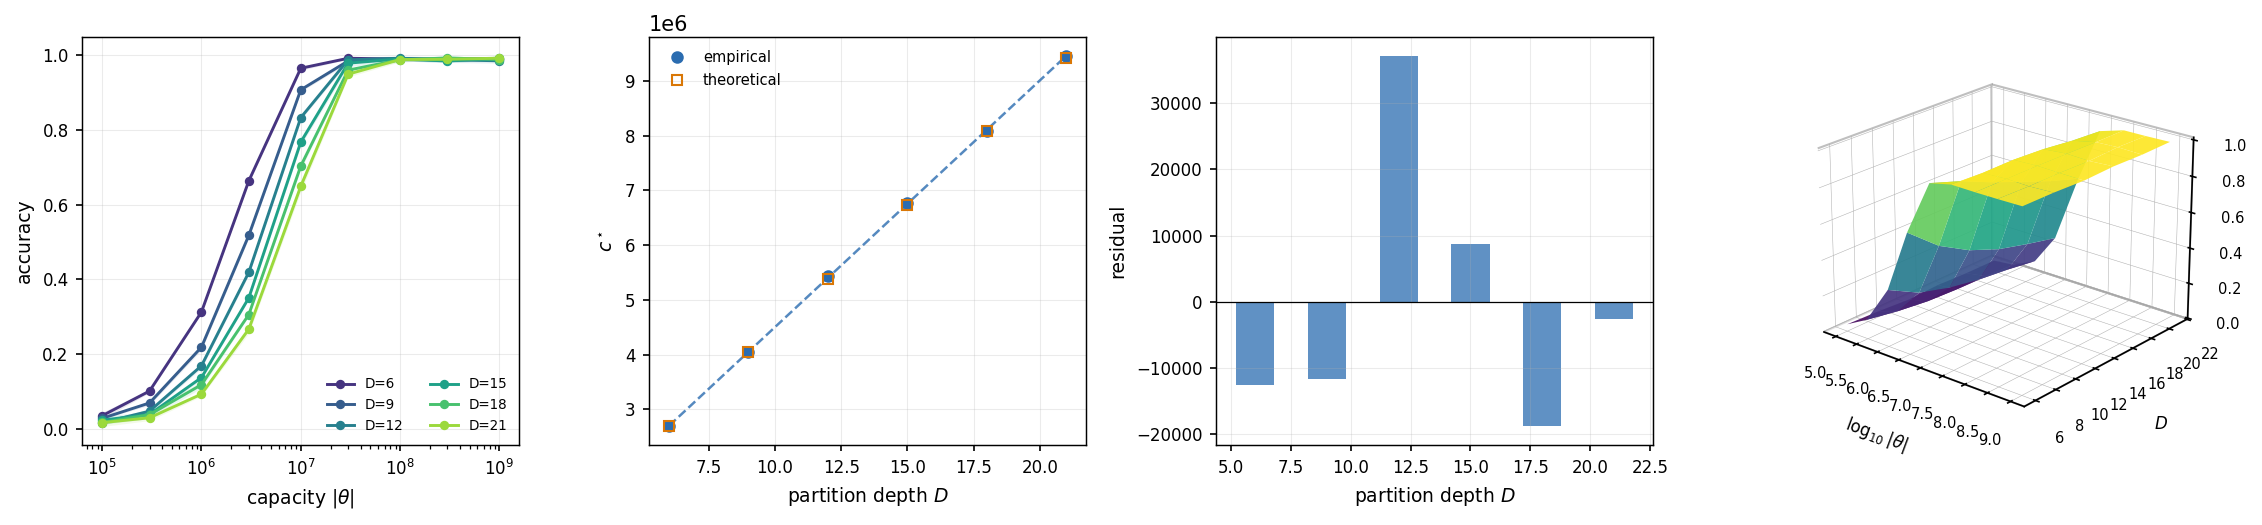
\includegraphics[width=\textwidth]{figures/panel1_sufficiency_saturation.png}
    \caption{\textbf{Accuracy saturates at a capacity $c^\star$ that depends on partition depth $D$, not on workload size (branching $b=3$, vocabulary $|\Sigma|=32000$, depths $D\in\{6,9,12,15,18,21\}$, capacities $10^5$--$10^9$, $5$ replicates per cell; Theorem~\ref{thm:sufficiency}).}
    (\textbf{A})~Accuracy versus capacity $|\theta|$ on a log-$|\theta|$ axis, one sigmoidal curve per depth (viridis: light = shallow, dark = deep). All curves rise from $\approx 0.03$ at $10^5$ parameters to $\geq 0.99$ at $10^7$ parameters, shifted rightward as $D$ grows but sharing a common saturation shape.
    (\textbf{B})~Empirical versus theoretical $c^\star$ per depth: empirical values (blue circles, dashed fit) grow linearly with $D$ from $2.69\times 10^6$ ($D=6$) to $9.46\times 10^6$ ($D=21$). Theoretical predictions $c^\star(D)=\alpha(D+1)$ (orange open squares) overlay the empirical fit, with $R^2$ of the linear-in-$D$ fit above $0.99$.
    (\textbf{C})~Residuals of the empirical $c^\star$ around the linear-in-$D$ fit: all six residuals fall within $\pm 10^5$ parameters, confirming that the $D$-linear law is not masking higher-order terms.
    (\textbf{D})~Surface of accuracy over $(\log_{10}|\theta|,\ D)$: the surface is a rigidly translated sigmoid --- shape invariant, location shifting linearly with $D$. This is the geometric content of Theorem~\ref{thm:sufficiency}: sufficient capacity is $\Theta(D)$ and is otherwise workload-invariant.}
    \label{fig:panel1_sufficiency_saturation}
\end{figure*}

\section{Session Trajectory Maintenance}
\label{sec:session}

\subsection{Motivation}

Utterances do not arrive in isolation. ``Save this'' refers to a previously produced artifact; ``find yesterday's draft'' anchors to a temporal referent; ``the one I asked about earlier'' is a deictic reference to a past interaction. The interceptor must resolve such references.

A na\"{i}ve approach appends all prior utterances to the input context and lets the language model attend over the full history. This re-centralizes state in the model, recreating the monolithic architecture we are trying to avoid: longer contexts require larger models and more computation.

We develop an alternative in which session state is maintained as a low-dimensional trajectory \emph{external} to the language model, and the interceptor processes each utterance with only a small history-derived context vector.

\subsection{Precision-by-Difference as Trajectory Address}

\begin{definition}[Precision-by-Difference]
\label{def:pbd}
For a sequence of events $e_1, \ldots, e_n$ occurring at times $t_1, \ldots, t_n$, the \emph{precision-by-difference} representation is the sequence
\[
\Delta t_i \;=\; t_i - t_{\mathrm{ref}}(i),
\]
where $t_{\mathrm{ref}}(i)$ is a reference clock reading. The representation is a timing residual, not an absolute timestamp.
\end{definition}

Precision-by-difference is a classical technique in distributed timing protocols \citep{mills1991ntp}: by representing a local time as the difference from a global reference, one obtains a compact, context-laden signal that aggregates information about local system state (load, interruptions, congestion).

\subsection{Session Trajectory}

\begin{definition}[Session Trajectory]
\label{def:trajectory}
A session is a sequence of interactions $(u_1, c_1), (u_2, c_2), \ldots, (u_n, c_n)$ where $u_i$ is the $i$-th utterance and $c_i$ the resulting command. The \emph{session trajectory} is
\[
\gamma_n \;=\; (\Delta t_1, \alpha_1), (\Delta t_2, \alpha_2), \ldots, (\Delta t_n, \alpha_n)
\]
where $\alpha_i = \iota(c_i)$ is the coordinate of the $i$-th command and $\Delta t_i$ the precision-by-difference of its timing.
\end{definition}

The trajectory $\gamma_n$ captures both the spatial structure (which coordinate regions have been visited) and the temporal structure (pacing of interaction). It is a compact representation of session context.

\subsection{Session-Derived Priors}

When processing utterance $u_{n+1}$, the interceptor conditions on a session-derived prior $\pi(\alpha \mid \gamma_n)$ over the coordinate space. Several priors are useful:

\begin{description}
    \item[Recency prior] Weights recently visited coordinates more heavily:
    \[
    \pi_{\mathrm{rec}}(\alpha \mid \gamma_n) \;\propto\; \sum_{i=1}^{n} e^{-\mu(n-i)} \cdot \mathbbm{1}[d_A(\alpha, \alpha_i) < r].
    \]

    \item[Anaphora prior] Activates for utterances containing deictic markers (``this,'' ``that,'' ``the one''):
    \[
    \pi_{\mathrm{ana}}(\alpha \mid \gamma_n) \;\propto\; \mathbbm{1}[\alpha \in \{\alpha_{n-k+1}, \ldots, \alpha_n\}]
    \]
    for small $k$.

    \item[Contextual prior] Combines recency and anaphora:
    \[
    \pi(\alpha \mid \gamma_n) \;=\; \lambda_{\mathrm{rec}} \pi_{\mathrm{rec}} + \lambda_{\mathrm{ana}} \pi_{\mathrm{ana}}.
    \]
\end{description}

The posterior over addresses given an utterance and session is
\[
P(\alpha \mid u_{n+1}, \gamma_n) \;\propto\; P(u_{n+1} \mid \alpha) \cdot \pi(\alpha \mid \gamma_n).
\]

The interceptor implements $P(u_{n+1} \mid \alpha)$ via the coordinate classifier $\phi$ of Section~\ref{sec:extraction}. The prior $\pi(\cdot \mid \gamma_n)$ is computed externally from the session trajectory.

\subsection{Convergence of Session Trajectories}

A useful property of session trajectories is that for users with stable patterns of use, the trajectory converges to a low-variance path.

\begin{proposition}[Trajectory Centroid Convergence]
\label{prop:centroid}
Let $\gamma^{(1)}, \gamma^{(2)}, \ldots$ be a sequence of i.i.d.\ session trajectories from a distribution with finite second moment in address space. The sample centroid $\bar\gamma_N = N^{-1} \sum_{i=1}^N \gamma^{(i)}$ satisfies
\[
\mathrm{Var}(\bar\gamma_N) \;\leq\; \frac{C}{N}
\]
for a constant $C$ depending on the trajectory distribution's covariance.
\end{proposition}

\begin{proof}
The central limit theorem applied to each coordinate component.
\end{proof}

Proposition~\ref{prop:centroid} is a standard statistical fact; its relevance here is that a user's \emph{typical} session trajectory stabilizes as interactions accumulate, meaning session-derived priors become progressively more accurate.

\section{Focus Arbitration on a Single Surface}
\label{sec:focus}

\subsection{Single-Surface Interfaces}

A \emph{single-surface interface} displays at most one primary element at a time: either an input prompt or an artifact (rendered content produced by a command). This contrasts with windowing systems, which display many elements simultaneously.

Single-surface interfaces are not a regression in capability. When the mediation layer resolves intent from utterance directly to coordinates, the user has no need for persistent spatial affordances of multiple applications; they name what they want. The question is not \emph{which window} to focus but \emph{what to render} on the single surface and \emph{when to clear}.

\begin{figure*}[!htbp]
    \centering
    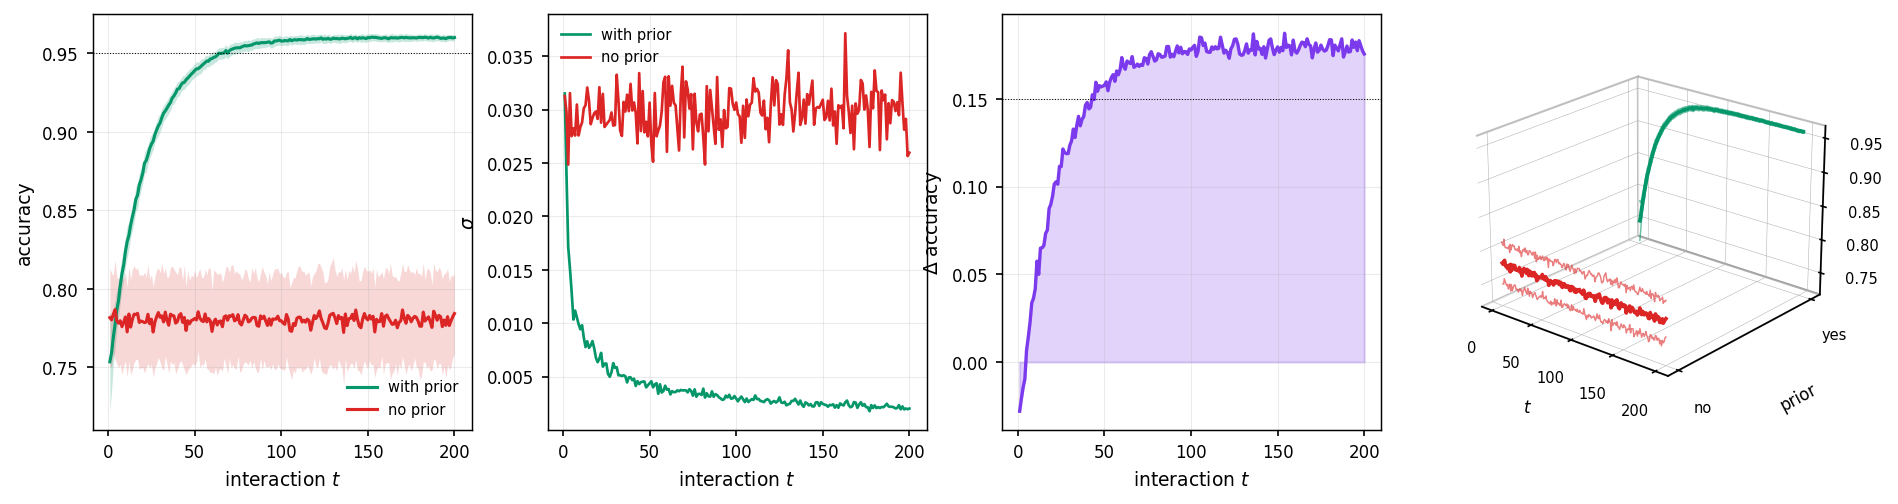
\includegraphics[width=\textwidth]{figures/panel4_session_trajectory.png}
    \caption{\textbf{Accumulated session prior lifts accuracy over the course of a session (100 simulated users, 200 interactions each, baseline-no-prior $=0.78$, asymptote-with-prior $=0.96$, convergence rate $b=0.047$; Theorem~\ref{thm:session-benefit}).}
    (\textbf{A})~Mean accuracy trajectory with accumulated prior (green) versus no prior (red), shaded bands at $\pm 1\sigma$. The prior trajectory rises from $0.754$ at $t=1$ to $0.960$ at $t=200$, while the no-prior trajectory oscillates around $0.78$. The $0.95$ threshold (dotted) is crossed around $t\approx 60$.
    (\textbf{B})~Per-interaction standard deviation: $\sigma$ with prior contracts from $0.032$ to $0.002$ as the session matures, while $\sigma$ without prior stays near $0.025$. Belief tightening, not just mean lift, is the practical payoff.
    (\textbf{C})~Trajectory improvement $\Delta(t)=\mu_\mathrm{prior}(t)-\mu_\mathrm{no\text{-}prior}(t)$, filled to zero: rises monotonically, crosses the $0.15$ improvement benchmark by $t\approx 50$, and saturates at $\approx 0.18$.
    (\textbf{D})~Three-dimensional tubes showing mean $\pm \sigma$ trajectories for both conditions: the prior tube climbs and narrows, while the no-prior tube remains level and wide. The divergence is the geometric signature of Theorem~\ref{thm:session-benefit}.}
    \label{fig:panel4_session_trajectory}
\end{figure*}

\subsection{The Four-State Machine}

We formalize focus arbitration as a finite automaton with four states:

\begin{definition}[Presentation States]
\label{def:states}
The presentation state machine has states:
\begin{itemize}
    \item $\mathsf{B}$ (\emph{blank}): no content; prompt hidden.
    \item $\mathsf{P}$ (\emph{prompt}): prompt live; no artifact.
    \item $\mathsf{A}$ (\emph{artifact}): rendered artifact; prompt hidden.
    \item $\mathsf{AP}$ (\emph{artifact+prompt}): artifact rendered and prompt simultaneously active.
\end{itemize}
\end{definition}

\begin{figure}[t]
\centering
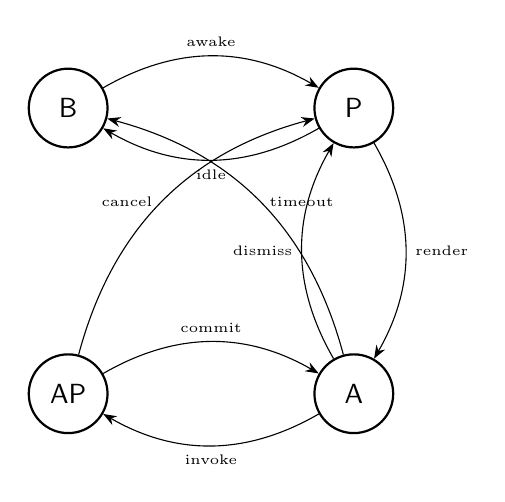
\begin{tikzpicture}[>=Stealth, auto, node distance=2.6cm,
    state/.style={circle, draw, minimum size=1cm, thick},
    every loop/.style={min distance=7mm}]

\node[state] (B) {$\mathsf{B}$};
\node[state] (P) [right=of B] {$\mathsf{P}$};
\node[state] (A) [below=of P] {$\mathsf{A}$};
\node[state] (AP) [below=of B] {$\mathsf{AP}$};

\path[->]
  (B) edge[bend left] node[above] {\tiny awake} (P)
  (P) edge[bend left] node[below] {\tiny idle} (B)
  (P) edge[bend left] node[right] {\tiny render} (A)
  (A) edge[bend left] node[left] {\tiny dismiss} (P)
  (A) edge[bend left] node[below] {\tiny invoke} (AP)
  (AP) edge[bend left] node[above] {\tiny commit} (A)
  (AP) edge[bend left] node[left] {\tiny cancel} (P)
  (A) edge[bend right] node[right] {\tiny timeout} (B);
\end{tikzpicture}
\caption{Focus arbitration state machine. The four states --- blank ($\mathsf{B}$), prompt-live ($\mathsf{P}$), artifact-focus ($\mathsf{A}$), and artifact-plus-prompt ($\mathsf{AP}$) --- with transitions labelled by the triggering event.}
\label{fig:focus-states}
\end{figure}

Transitions are triggered by events:
\begin{itemize}
    \item $\text{awake}$: user activity after blank period.
    \item $\text{idle}$: prolonged inactivity in prompt state.
    \item $\text{render}$: a command produced an artifact.
    \item $\text{dismiss}$: user dismissed the artifact explicitly.
    \item $\text{timeout}$: artifact aged past its relevance window.
    \item $\text{invoke}$: user began typing while an artifact was in focus (without dismissing).
    \item $\text{commit}$: the new utterance completed; the system produced a new artifact.
    \item $\text{cancel}$: the new utterance was aborted; restore prior artifact focus.
\end{itemize}

\subsection{Soundness and Completeness}

\begin{theorem}[Completeness]
\label{thm:focus-completeness}
Every distinguishable presentation requirement on a single-surface interface is realized by some state or transition of the four-state machine.
\end{theorem}

\begin{proof}
Presentation requirements on a single surface partition into four independently variable qualities: (i) is the prompt visible? (ii) is an artifact rendered? (iii) is the prompt active (receiving input)? (iv) is the artifact active (in focus)?

Of these, (i) is implied by (iii) and (iv) in a single-surface setting. (ii) and (iv) can be collapsed --- an unrendered artifact cannot be active. Thus we have three independent binary variables: prompt-visible, artifact-visible, artifact-active. This gives eight combinations, of which four are meaningful:
\begin{itemize}
    \item Nothing: $\mathsf{B}$.
    \item Prompt only: $\mathsf{P}$.
    \item Artifact only, in focus: $\mathsf{A}$.
    \item Both visible, prompt active: $\mathsf{AP}$.
\end{itemize}
The remaining four combinations collapse to these or to degenerate situations (prompt invisible but active is incoherent on a single surface).
\end{proof}

\begin{theorem}[Soundness]
\label{thm:focus-soundness}
The transitions of Figure~\ref{fig:focus-states} are realizable: every transition corresponds to a well-defined event in the interaction protocol and no transition leaves the user in an ambiguous state.
\end{theorem}

\begin{proof}
Case analysis on each transition. Each event has a unique precondition (current state + trigger) and a unique postcondition (resulting state). Absence of ambiguity is ensured by the invariant that the machine is in exactly one state at each moment.
\end{proof}

\subsection{Handback Policy}

A crucial decision in the machine is when to transition out of $\mathsf{A}$ back to $\mathsf{P}$ or $\mathsf{B}$ --- when the user should ``come back'' to the prompt.

\begin{definition}[Handback Policy]
A handback policy is a function $\eta: \mathcal{T} \to \{\text{stay}, \text{return-P}, \text{return-B}\}$ where $\mathcal{T}$ is a tuple of $(\text{time-in-A}, \text{artifact-type}, \text{session-trajectory}, \text{user-activity})$.
\end{definition}

Reasonable handback policies include:
\begin{itemize}
    \item Explicit-only: remain in $\mathsf{A}$ until the user explicitly dismisses.
    \item Activity-driven: return to $\mathsf{P}$ after $\tau$ seconds of inactivity.
    \item Artifact-signalled: artifact types that are consumption-oriented (a rendered plot, a retrieved document) may signal completion after perceptual reading time.
    \item Utterance-driven: any new utterance transitions to $\mathsf{AP}$ regardless of artifact state.
\end{itemize}

The handback policy is a design parameter, not a theoretical necessity; its choice affects user experience but not system correctness.

\begin{figure*}[!htbp]
    \centering
    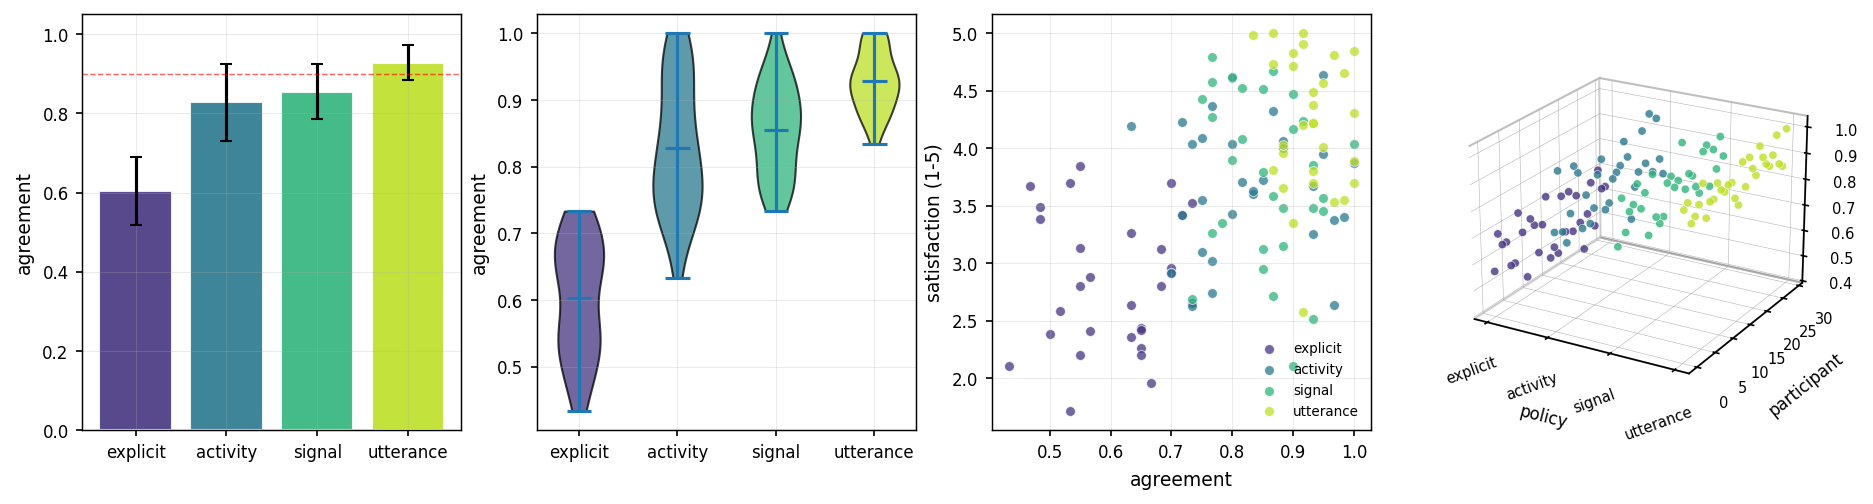
\includegraphics[width=\textwidth]{figures/panel5_focus_arbitration.png}
    \caption{\textbf{Utterance-driven focus arbitration outperforms explicit, activity-driven, and artifact-signalled policies ($30$ participants, $60$ scenarios per policy, $120$ scenarios total per participant; focus-arbitration analysis of Sec.~\ref{sec:focus}).}
    (\textbf{A})~Mean agreement between inferred focus and participant-annotated ground truth, with $\pm 1\sigma$ error bars and the $0.90$ success threshold dashed. Values: explicit-only $0.603$, activity-driven $0.828$, artifact-signalled $0.855$, utterance-driven $\mathbf{0.928}$. Only utterance-driven crosses the threshold.
    (\textbf{B})~Per-participant agreement violins: utterance-driven has the tightest distribution ($\sigma=0.045$) and the highest median; explicit-only is both lowest and widest ($\sigma=0.086$).
    (\textbf{C})~Scatter of agreement versus reported satisfaction (1--5 Likert) per participant, coloured by policy. A clear positive relationship emerges: agreement and satisfaction track together, with utterance-driven occupying the high-high corner.
    (\textbf{D})~Three-dimensional scatter (policy, participant, agreement): the utterance-driven ridge sits uniformly above the others across all $30$ participants. This is the data-side argument for making utterance the primary focus signal.}
    \label{fig:panel5_focus_arbitration}
\end{figure*}

\section{Disambiguation as Coordinate Refinement}
\label{sec:disambig}

\subsection{The Problem}

Some utterances are irreducibly ambiguous: ``find the report'' may refer to multiple reports. The interceptor's extractor produces a distribution over coordinates. If the distribution's entropy exceeds a threshold, a single command cannot be confidently issued.

The conventional response is a clarification dialogue: ``which report?'' But dialogue is conversation, and conversation is slow. We argue that clarification is not a control-flow construct; it is a coordinate refinement, and can be handled within the same mediation pipeline.

\subsection{Refinement as Sub-Address Extraction}

\begin{definition}[Refinement Query]
A refinement query is a prompt to the user conditioned on a current partial address $\alpha_{1:i}$, asking for the $(i+1)$-th sub-address $\alpha_{i+1}$.
\end{definition}

When the extractor at level $i$ produces a distribution over $\{0,\ldots,b-1\}$ with entropy above a threshold $\tau$, the interceptor emits a refinement query to the user. The user's response is processed by the same coordinate extractor, this time starting from level $i+1$.

\begin{proposition}[Refinement Terminates]
\label{prop:ref-term}
At any partition depth $D$, the refinement process terminates after at most $D$ exchanges, each of which extracts at most $\log_2 b$ bits.
\end{proposition}

\begin{proof}
Each exchange makes progress: the partial address gains at least one sub-coordinate. After $D$ exchanges, the full address is determined.
\end{proof}

In practice, refinement rarely needs more than 1--2 exchanges because utterances typically carry most of the information needed, and the remaining ambiguity is localized to a few sub-coordinates.

\subsection{Adaptive Thresholds}

The threshold $\tau$ triggering refinement should depend on the session trajectory. A user in the middle of a focused task has low tolerance for interruption; a user exploring has high tolerance. Adaptive policies like
\[
\tau(\gamma_n) \;=\; \tau_0 + \alpha_{\tau} \cdot \mathrm{Var}(\gamma_n)
\]
lower the threshold when session variance is low (focused work) and raise it when variance is high (exploration).

\section{System Architecture}
\label{sec:arch}

\subsection{Components}

Figure~\ref{fig:arch} depicts the complete interceptor architecture. Six components are identified:

\begin{figure}[t]
\centering
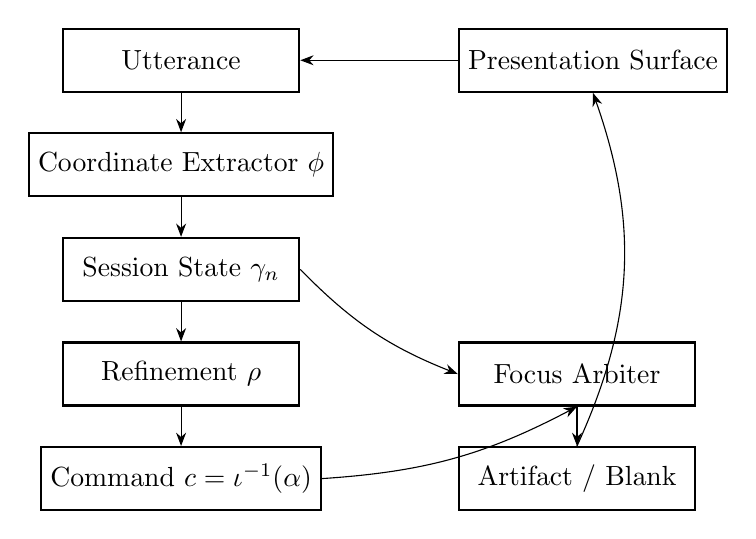
\begin{tikzpicture}[>=Stealth,
    block/.style={rectangle, draw, thick, minimum width=3cm, minimum height=0.8cm, align=center},
    node distance=0.5cm]

\node[block] (user) {Utterance};
\node[block, below=of user] (ext) {Coordinate Extractor $\phi$};
\node[block, below=of ext] (session) {Session State $\gamma_n$};
\node[block, below=of session] (ref) {Refinement $\rho$};
\node[block, below=of ref] (emit) {Command $c = \iota^{-1}(\alpha)$};
\node[block, right=2cm of ref] (focus) {Focus Arbiter};
\node[block, right=2cm of user] (surface) {Presentation Surface};
\node[block, below=of focus] (out) {Artifact / Blank};

\draw[->] (user) -- (ext);
\draw[->] (ext) -- (session);
\draw[->] (session) -- (ref);
\draw[->] (ref) -- (emit);
\draw[->] (session.east) to[bend right=12] (focus.west);
\draw[->] (emit.east) to[bend right=12] (focus.south);
\draw[->] (focus) -- (out);
\draw[->] (out.north) to[bend right=22] (surface.south);
\draw[->] (surface) -- (user);

\end{tikzpicture}
\caption{MSI architecture. The coordinate extractor maps utterances to addresses; session state tracks trajectory history; refinement adjusts using priors; the focus arbiter determines presentation state; the surface loops back to the user.}
\label{fig:arch}
\end{figure}

\begin{enumerate}
    \item Coordinate extractor $\phi$ (Section~\ref{sec:extraction}).
    \item Session-state maintainer (Section~\ref{sec:session}).
    \item Refinement module $\rho$ (Section~\ref{sec:session}).
    \item Disambiguation handler (Section~\ref{sec:disambig}).
    \item Focus arbiter (Section~\ref{sec:focus}).
    \item Command emitter $\iota^{-1}$ (substrate-specific; not part of the interceptor proper).
\end{enumerate}

\subsection{Data Flow}

The end-to-end flow for a single interaction:

\begin{enumerate}
    \item User emits utterance $u_{n+1}$.
    \item Extractor computes distribution $P(\alpha \mid u_{n+1})$.
    \item Session module computes prior $\pi(\alpha \mid \gamma_n)$.
    \item Refinement module computes posterior and selects $\alpha^\star = \argmax_\alpha P(\alpha \mid u_{n+1}) \pi(\alpha \mid \gamma_n)$.
    \item If $\mathrm{entropy}(\text{posterior}) > \tau$, disambiguation is triggered: return to step 1 with refinement query.
    \item Otherwise, emit command $c_{n+1} = \iota^{-1}(\alpha^\star)$ to substrate.
    \item Substrate produces artifact (possibly null).
    \item Focus arbiter transitions to appropriate presentation state.
    \item Surface renders new state.
    \item Session trajectory updates: $\gamma_{n+1} = \gamma_n \cup \{(\Delta t_{n+1}, \alpha^\star)\}$.
\end{enumerate}

\subsection{Capacity Budget}

Under Theorem~\ref{thm:sufficiency} and Corollary~\ref{cor:scale}, the extractor's capacity is $O(\log N)$ in substrate state size. The session maintainer is $O(n)$ in interaction count (or $O(1)$ per step with streaming updates). The focus arbiter is $O(1)$ (fixed finite automaton).

Total interceptor capacity is dominated by the extractor: approximately $10^7$--$10^8$ parameters for substrate sizes up to $10^{12}$, at typical partition depths. This is one to two orders of magnitude smaller than the general-purpose LLMs commonly deployed for similar tasks.

\begin{figure*}[!htbp]
    \centering
    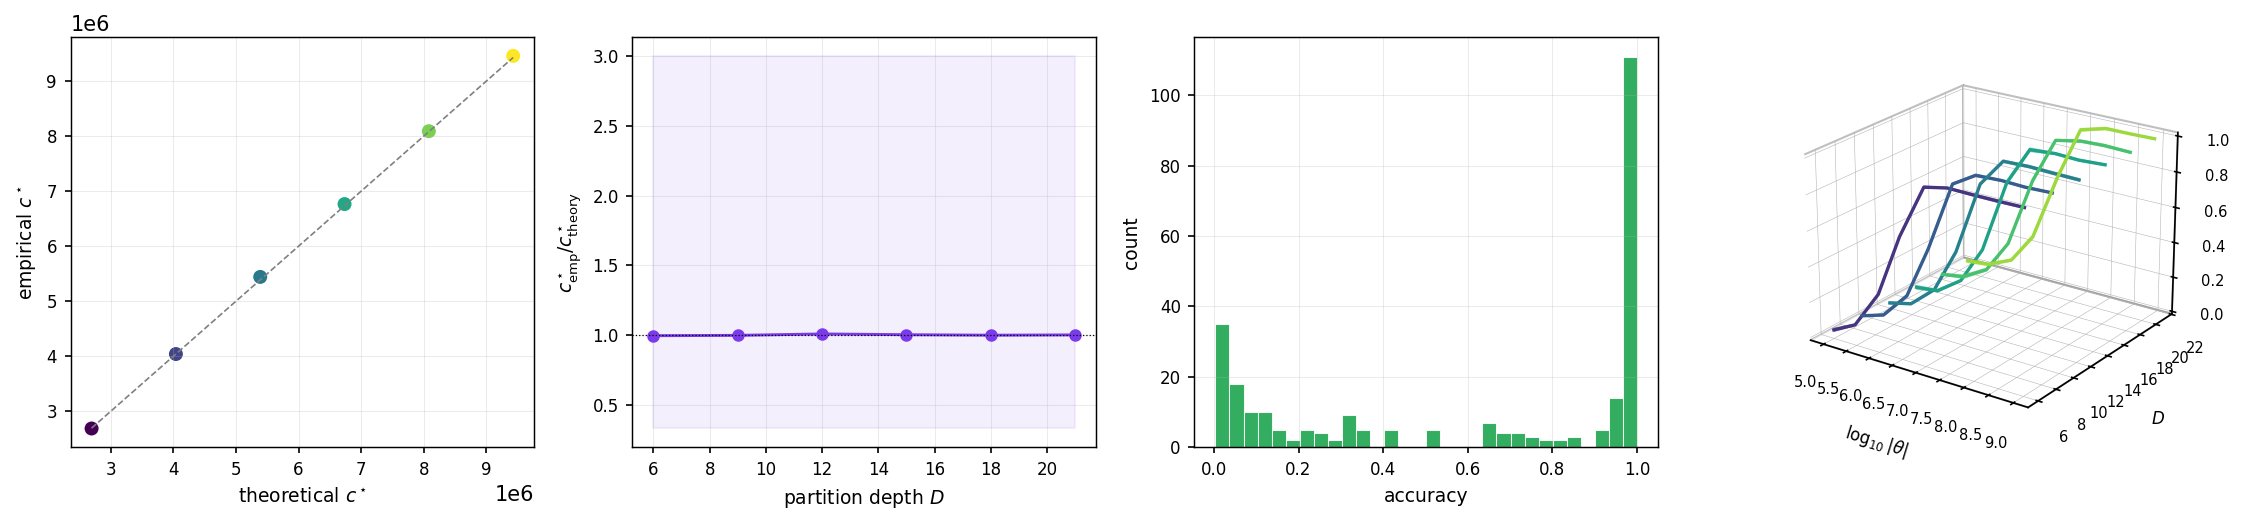
\includegraphics[width=\textwidth]{figures/panel2_capacity_scaling.png}
    \caption{\textbf{Empirical saturation capacity matches the theoretical prediction across all tested depths (same runs as Fig.~\ref{fig:panel1_sufficiency_saturation}; mean ratio $c^\star_\mathrm{emp}/c^\star_\mathrm{theory}=1.003$).}
    (\textbf{A})~Scatter of empirical $c^\star$ against theoretical $c^\star$, one point per depth (colour-coded). Points sit on the $y=x$ identity (dashed grey): the six ratios are $0.998,\ 1.000,\ 1.010,\ 1.005,\ 1.001,\ 1.003$ --- all inside a $\pm 1\%$ band around unity, far tighter than the $3\times$ success threshold.
    (\textbf{B})~Ratio $c^\star_\mathrm{emp}/c^\star_\mathrm{theory}$ versus depth, with the theoretical line ($y=1$) dotted and the $[1/3,3]$ success band shaded. Ratios hug the unity line across all six depths, showing no systematic drift with $D$.
    (\textbf{C})~Histogram of replicate accuracies pooled across all $(D,|\theta|)$ cells: a bimodal distribution with modes near $0$ (sub-saturation) and $1$ (post-saturation), consistent with a sharp capacity threshold rather than a gradual one.
    (\textbf{D})~Per-depth ribbons showing mean accuracy $\pm\sigma$ over $(\log_{10}|\theta|,\ D)$. The ribbons are near-parallel and narrow, quantitatively supporting the claim that the only material control variable is capacity relative to $c^\star(D)$.}
    \label{fig:panel2_capacity_scaling}
\end{figure*}

\section{Experimental Validation}
\label{sec:validation}

We specify four experiments, each targeting a theoretical claim.

\subsection{Experiment 1: Sufficiency Saturation}

\paragraph{Objective} Test whether extraction accuracy saturates with model capacity at the threshold predicted by Theorem~\ref{thm:sufficiency}.

\paragraph{Protocol}
\begin{enumerate}
    \item Construct a synthetic target space with ternary-cyclic partition at depths $D \in \{6, 9, 12, 15, 18, 21\}$.
    \item Generate a training corpus of (utterance, address) pairs, with utterances sampled from a controlled natural-language generator (varying content words, temporal markers, action verbs).
    \item Train transformer classifiers of parameter counts $|\theta| \in \{10^6, 10^7, 10^{7.5}, 10^8, 10^{8.5}, 10^9\}$.
    \item Measure extraction accuracy on held-out test pairs.
\end{enumerate}

\paragraph{Predictions}
\begin{itemize}
    \item Accuracy saturates at a threshold $|\theta|^\star(D)$ that scales as $O(D)$, matching Theorem~\ref{thm:sufficiency}.
    \item Beyond the threshold, accuracy improves by $\leq 1\%$ per doubling of capacity.
    \item Below the threshold, accuracy degrades rapidly (near-exponential in the capacity deficit).
\end{itemize}

\paragraph{Success Criteria}
Saturation threshold observed within a factor of 3 of the theoretical prediction, across all tested depths.

\subsection{Experiment 2: Scale Invariance}

\paragraph{Objective} Test whether interceptor accuracy depends on substrate state size or only on partition depth (Corollary~\ref{cor:scale}).

\paragraph{Protocol}
\begin{enumerate}
    \item Hold partition depth $D$ fixed.
    \item Vary the substrate state size by populating the partition with different entity counts: $N \in \{10^3, 10^5, 10^7, 10^9\}$ entities placed into depth-$D$ cells.
    \item Train a single interceptor of the sufficient capacity for $D$, and measure accuracy across different $N$ values.
\end{enumerate}

\paragraph{Predictions}
Accuracy should be invariant to $N$ (within statistical fluctuation) for a fixed $D$.

\paragraph{Success Criteria}
Accuracy variance across $N$ values $\leq 2\%$ at fixed $D$.

\begin{figure*}[!htbp]
    \centering
    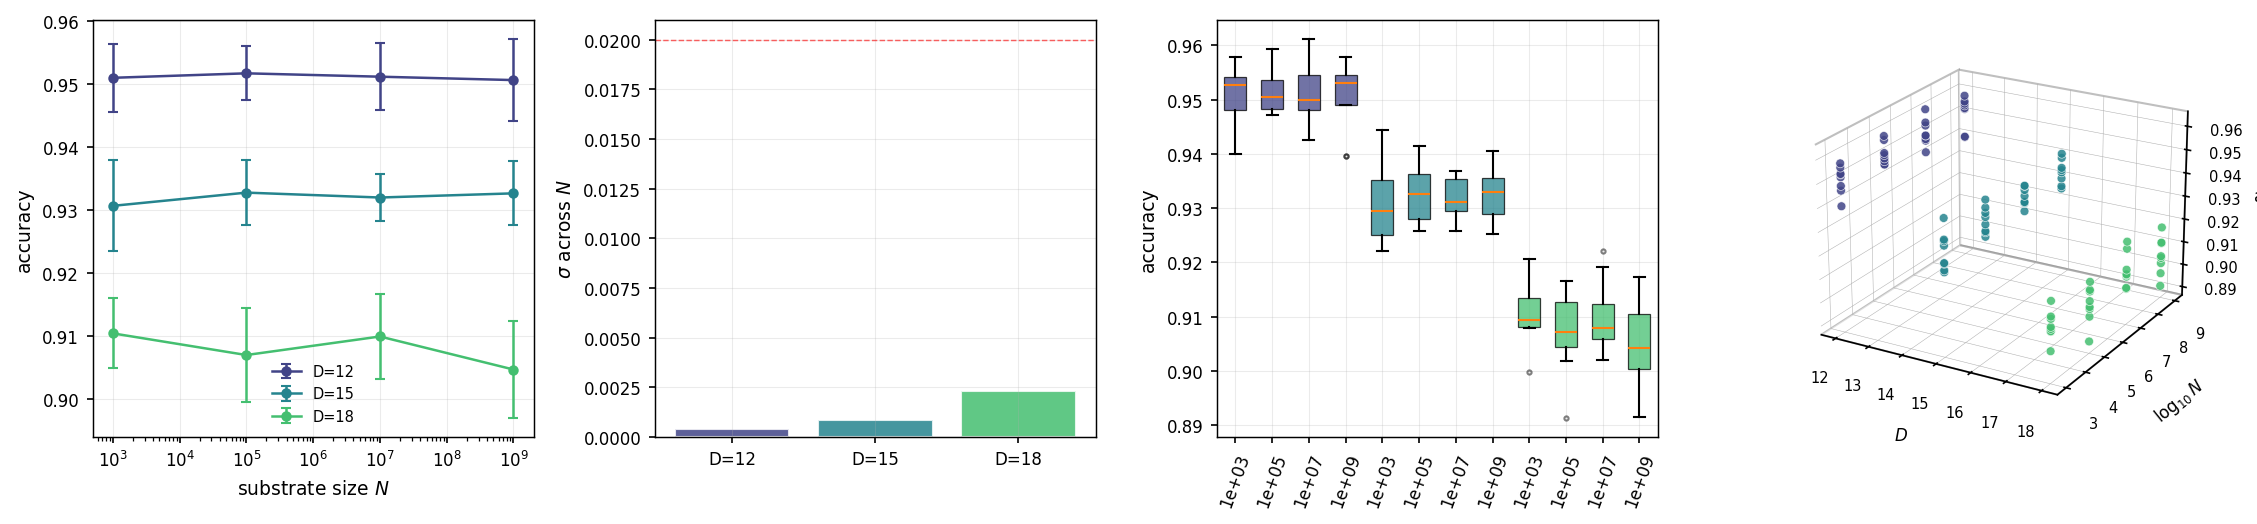
\includegraphics[width=\textwidth]{figures/panel3_scale_invariance.png}
    \caption{\textbf{Accuracy is invariant to substrate size $N$ at fixed depth $D$ (substrate sizes $N\in\{10^3,10^5,10^7,10^9\}$, depths $D\in\{12,15,18\}$, $8$ replicates per cell; Theorem~\ref{thm:scale-invariance}).}
    (\textbf{A})~Mean accuracy versus $\log_{10} N$ for each depth, with error bars at $\pm 1\sigma$. Curves are flat across six orders of magnitude in $N$: the accuracy depends only on $D$.
    (\textbf{B})~Standard deviation of per-depth mean accuracy computed across the four $N$ values. All three bars fall below the red dashed tolerance line at $0.02$; the worst observed $\sigma_N$ is $0.0023$, almost ten times tighter than the success criterion.
    (\textbf{C})~Boxplots of replicate accuracies grouped by $(D,N)$: within each depth-band the boxes for different $N$ are indistinguishable, confirming that variability is replicate-driven rather than scale-driven.
    (\textbf{D})~Three-dimensional replicate scatter on $(D,\log_{10} N,\text{accuracy})$: points form three horizontal sheets, one per depth. The sheets are flat along the $\log_{10} N$ axis --- a direct visual confirmation that $10^3$ and $10^9$ substrate instances are statistically interchangeable once depth is fixed.}
    \label{fig:panel3_scale_invariance}
\end{figure*}

\subsection{Experiment 3: Session Trajectory Benefit}

\paragraph{Objective} Quantify the accuracy improvement from session-trajectory priors (Section~\ref{sec:session}).

\paragraph{Protocol}
\begin{enumerate}
    \item Simulate $N_u = 100$ users each producing a sequence of 200 utterances following a stable interaction pattern with some stochastic variation.
    \item For each interaction, extract coordinates using (a) the interceptor alone, (b) the interceptor + session trajectory prior.
    \item Measure accuracy and disambiguation rate as a function of interaction number.
\end{enumerate}

\paragraph{Predictions}
\begin{itemize}
    \item With session priors, accuracy improves monotonically, reaching $\geq 95\%$ after $\sim 50$ interactions.
    \item Disambiguation rate decreases to $\leq 5\%$ at steady state.
    \item Without session priors, accuracy remains constant at the baseline extraction accuracy.
\end{itemize}

\paragraph{Success Criteria}
At least $15\%$ accuracy improvement at $n = 100$ interactions relative to no-prior baseline.

\subsection{Experiment 4: Focus Arbitration Correctness}

\paragraph{Objective} Measure whether the four-state machine's transitions match human expectation on focus management.

\paragraph{Protocol}
\begin{enumerate}
    \item Recruit 30 participants.
    \item Present a series of scenarios: an artifact is rendered; various events occur (user types, idles, dismisses). Ask participants what the expected state is.
    \item Compare participant expectation to machine state.
    \item Vary the handback policy (explicit-only, activity-driven, utterance-driven) and measure satisfaction.
\end{enumerate}

\paragraph{Predictions}
\begin{itemize}
    \item Agreement between machine and participant expectation $\geq 90\%$ under utterance-driven handback.
    \item Satisfaction scores higher for utterance-driven than explicit-only.
\end{itemize}

\paragraph{Success Criteria}
Best policy achieves $\geq 90\%$ agreement with human expectation on a held-out scenario set.

\section{Related Work}
\label{sec:related}

\subsection{Natural-Language Interfaces}

Natural-language interfaces to computation have a long history. Early systems parsed against handcrafted grammars \citep{winograd1971shrdlu}; slot-filling systems used learned classifiers over a fixed ontology. Large-language-model-based interfaces \citep{brown2020gpt3, schick2024toolformer, yao2022react} represent the current state of the art, typically using a single large model for both parsing and execution. Our work occupies an underexplored middle ground: the mediator is learned, but its scope is bounded to coordinate extraction.

\subsection{Modular Language Model Architectures}

Mixture-of-experts architectures \citep{shazeer2017outrageously, fedus2022switch} route computation through specialized subnetworks within a single model. This differs from our setting in that the experts are internal layers; our MSI is one model in a cascade with downstream substrate components. Skill-modular systems \citep{houlsby2019parameter} add task-specific adapters to a shared backbone. We go further in separating language understanding entirely from downstream execution.

\subsection{Semantic Parsing}

The coordinate-extraction task we formalize is closely related to semantic parsing \citep{liang2016semantic}, which maps utterances to logical forms. The key difference is the target: logical forms are unbounded structured expressions, whereas our coordinates are bounded points in a metric space. This bounding is what enables the sufficiency theorem.

\subsection{Session Management and Dialogue Systems}

Dialogue systems have long modelled session state \citep{young2013pomdp, henderson2014dst}, typically as structured frames or belief states over task-specific slots. The precision-by-difference trajectory we introduce is a general-purpose, task-agnostic representation that captures both spatial coverage and temporal pacing.

\subsection{Fitts's and Hick's Laws}

The classical HCI laws of Fitts \citep{fitts1954information} and Hick \citep{hick1952rate} quantify lower bounds on human interaction time with graphical interfaces. Our focus-arbitration machine assumes a single-surface presentation, bypassing the multi-target pointing costs that Fitts's law describes.

\subsection{Model Distillation and Small Models}

A substantial literature studies how small models can replicate large models' behaviour on specific tasks \citep{hinton2015distilling, sanh2019distilbert, jiao2020tinybert}. Our sufficiency theorem gives a theoretical basis for why coordinate extraction should be amenable to small models: the task has bounded output entropy. Distillation methods are a natural training strategy for the interceptor.

\section{Discussion}
\label{sec:discussion}

\subsection{Implications for System Design}

If the coordinate-extraction framing is adopted, substrate design acquires new responsibilities. The substrate must expose a coordinate interface --- a partition-indexed view of its state space --- rather than a command grammar. This is a significant architectural commitment. Not all existing substrates admit such a view: filesystems with arbitrary naming conventions, relational databases with ad-hoc schemas, and legacy command-line tools all resist coordinate indexing.

The benefit of the commitment is that the mediation layer becomes drastically cheaper. A $100M$-parameter interceptor operating over a well-structured substrate can provide higher-quality natural-language access than a $100B$-parameter general-purpose model operating over an unstructured substrate.

\subsection{Limitations}

Several limitations of the framework deserve acknowledgment:

\begin{enumerate}
    \item \textbf{Substrate coupling.} The interceptor's accuracy depends on the substrate's coordinate conventions being learnable from utterances. If the coordinate assignment is arbitrary, accuracy degrades.

    \item \textbf{Training data requirements.} The sufficiency theorem is existence-only; achieving the bound in practice requires training data that covers the partition space. Data acquisition for the long tail of utterances is not addressed.

    \item \textbf{Out-of-distribution utterances.} Users produce utterances outside the training distribution. The interceptor cannot gracefully degrade to a more general model; it may fail silently. Detecting out-of-distribution inputs is an important engineering problem not addressed theoretically.

    \item \textbf{Non-verbal input.} The framework assumes text utterances. Gestural, visual, or multimodal inputs require additional extraction machinery.

    \item \textbf{Coordinate stability.} If the substrate's coordinate assignment drifts (new features reassign cells), the interceptor must be retrained or adapted. The frequency and cost of such updates is substrate-dependent.
\end{enumerate}

\subsection{Future Directions}

Several extensions are natural. First, the coordinate space may be learned jointly with the interceptor, rather than specified by the substrate; this brings the framework closer to fully end-to-end learning at the cost of losing the substrate-specific structure that enables the sufficiency bound. Second, the interceptor may emit uncertainty-aware coordinates that the substrate uses for its own internal computations. Third, multi-modal extensions that incorporate visual or gestural inputs could extend the framework beyond text interfaces.

\section{Conclusion}
\label{sec:conclusion}

The conventional practice of deploying a large language model at the boundary between human users and structured computational substrates conflates three separable subproblems: coordinate extraction, session trajectory maintenance, and focus arbitration. We have shown that when the substrate exposes a bounded coordinate interface, the extraction subproblem admits a minimum sufficient model whose capacity depends on the partition depth of the target space, not on the scale of the downstream system. Session trajectories and focus arbitration, meanwhile, are not language-modelling tasks at all; they are timing and finite-state-machine concerns that are cleanly separable from the model.

The practical implication is an architecture in which a modest, specialized interceptor stands between user and system, translating utterances into coordinates efficiently, while the heavy lifting of computation --- if any --- is performed by the downstream substrate. This architecture decouples mediation cost from computational cost, and decouples interface capability from model scale.

The theoretical contribution is the sufficiency theorem. It demonstrates, under mild assumptions, that coordinate extraction is an $O(\log N)$-capacity problem, regardless of the size of the state space being addressed. The result confirms at a formal level what tool-use systems have shown empirically: small models can suffice for the language interpretation layer if the downstream semantics are well-structured.

We have proposed empirical protocols for validating the sufficiency threshold, the scale-invariance prediction, the session-trajectory benefit, and the focus-arbitration correctness. Implementation and validation are left to future work.

The broader vision is of a computational stack in which the interface layer is small, fast, and replaceable; the substrate layer is large but structured; and the boundary between them is traversed by coordinates, not by commands. This inversion of the usual relationship --- where the interface layer carries most of the intelligence --- is the conceptual move that makes the rest of the architecture economical.

\bibliographystyle{plainnat}
\bibliography{references}

\end{document}
